\documentclass[UTF8,11pt]{ctexart}
\usepackage[a4paper,margin=22mm]{geometry}
\usepackage{amsmath,amssymb,bm,graphicx,adjustbox,fvextra,longtable,array}
\xeCJKDeclareCharClass{CJK}{"2160 -> "217F, "2460 -> "249B, "2200 -> "22FF}
\newcommand{\fitmath}[1]{\begin{adjustbox}{max width=\linewidth}$\displaystyle #1$\end{adjustbox}}
\setlength{\parindent}{0pt}\setlength{\parskip}{.65em}\renewcommand{\arraystretch}{1.3}
\sloppy\allowdisplaybreaks
\begin{document}
\section*{2023 年计算机统考 408 · 真题}
\subsection*{2023年全国硕士研究生入学统一考试}

\subsection*{计算机学科专业基础综合试题}

\subsection*{一、单项选择题（1～40小题，每小题2分，共80分。下列每小题给出的四个选项中，只有一项符合题目要求）}

1．下列对顺序存储的有序表（长度为n）实现给定操作的算法中，平均时间复杂度为O(1)的是\_\_\_\_\_\_。


\begin{center}\begin{tabular}{>{\raggedright\arraybackslash}p{\dimexpr(\linewidth-4\tabcolsep)/2\relax}>{\raggedright\arraybackslash}p{\dimexpr(\linewidth-4\tabcolsep)/2\relax}}
\textbf{A.} 查找包含指定值元素的算法 & \textbf{B.} 插入包含指定值元素的算法\\[.35em]
\textbf{C.} 删除第i（1≤i≤n）个元素的算法 & \textbf{D.} 获取第i（1≤i≤n）个元素的算法\\[.35em]\end{tabular}\end{center}

2．现有非空双向链表L，其结点结构为：


\begin{center}\begin{adjustbox}{max width=\linewidth}\begin{tabular}{|>{\raggedright\arraybackslash}p{\dimexpr(\linewidth-6\tabcolsep-4\arrayrulewidth)/3\relax}|>{\raggedright\arraybackslash}p{\dimexpr(\linewidth-6\tabcolsep-4\arrayrulewidth)/3\relax}|>{\raggedright\arraybackslash}p{\dimexpr(\linewidth-6\tabcolsep-4\arrayrulewidth)/3\relax}|}\hline
prev & data & next\\\hline\end{tabular}\end{adjustbox}\end{center}

prev 是指向直接前驱结点的指针， next 是指向直接后继结点的指针。若要在L 中指针p 所指向的结点（非尾结点）之后插入指针s 指向的新结点，则在执行了语句序列：“s->next=p->next; p->next=s”后，下列语句序列中还需要执行的是\_\_\_\_\_\_。


\begin{center}\begin{tabular}{>{\raggedright\arraybackslash}p{\dimexpr(\linewidth-4\tabcolsep)/2\relax}>{\raggedright\arraybackslash}p{\dimexpr(\linewidth-4\tabcolsep)/2\relax}}
\textbf{A.} s->next->prev=p; s->prev=p; & \textbf{B.} p->next->prev=s; s->prev=p;\\[.35em]
\textbf{C.} s->prev=s->next->prev; s->next->prev=s; & \textbf{D.} p->next->prev=s->prev; s->next->prev=p;\\[.35em]\end{tabular}\end{center}

3．若采用三元组表存储结构存储稀疏矩阵 M。则除三元组表外，下列数据中还需要保存的是\_\_\_\_\_\_。 I. M 的行数 II. M 中包含非零元素的行数 III. M 的列数 IV. M 中包含非零元素的列数


\begin{center}\begin{tabular}{>{\raggedright\arraybackslash}p{\dimexpr(\linewidth-8\tabcolsep)/4\relax}>{\raggedright\arraybackslash}p{\dimexpr(\linewidth-8\tabcolsep)/4\relax}>{\raggedright\arraybackslash}p{\dimexpr(\linewidth-8\tabcolsep)/4\relax}>{\raggedright\arraybackslash}p{\dimexpr(\linewidth-8\tabcolsep)/4\relax}}
\textbf{A.} 仅I、III & \textbf{B.} 仅I、IV & \textbf{C.} 仅II、IV & \textbf{D.} I、II、III、IV\\[.35em]\end{tabular}\end{center}

4．在由6 个字符组成的字符集S 中，各字符出现的频次分别为3, 4, 5, 6, 8, 10，为S 构造的哈夫曼编码的加权平均长度为\_\_\_\_\_\_。


\begin{center}\begin{tabular}{>{\raggedright\arraybackslash}p{\dimexpr(\linewidth-8\tabcolsep)/4\relax}>{\raggedright\arraybackslash}p{\dimexpr(\linewidth-8\tabcolsep)/4\relax}>{\raggedright\arraybackslash}p{\dimexpr(\linewidth-8\tabcolsep)/4\relax}>{\raggedright\arraybackslash}p{\dimexpr(\linewidth-8\tabcolsep)/4\relax}}
\textbf{A.} 2.\allowbreak{}4 & \textbf{B.} 2.\allowbreak{}5 & \textbf{C.} 2.\allowbreak{}67 & \textbf{D.} 2.\allowbreak{}75\\[.35em]\end{tabular}\end{center}

5．已知一棵二叉树的树形如下图所示，若其后序遍历为f, d, b, e, c, a，则其先 （前）序遍历序列是\_\_\_\_\_\_。


\begin{center}\begin{tabular}{>{\raggedright\arraybackslash}p{\dimexpr(\linewidth-8\tabcolsep)/4\relax}>{\raggedright\arraybackslash}p{\dimexpr(\linewidth-8\tabcolsep)/4\relax}>{\raggedright\arraybackslash}p{\dimexpr(\linewidth-8\tabcolsep)/4\relax}>{\raggedright\arraybackslash}p{\dimexpr(\linewidth-8\tabcolsep)/4\relax}}
\textbf{A.} a, e, d, f, b, c & \textbf{B.} a, c, e, b, d, f & \textbf{C.} c, a, b, e, f, d & \textbf{D.} d, f, e, b, a, c\\[.35em]\end{tabular}\end{center}

\begin{center}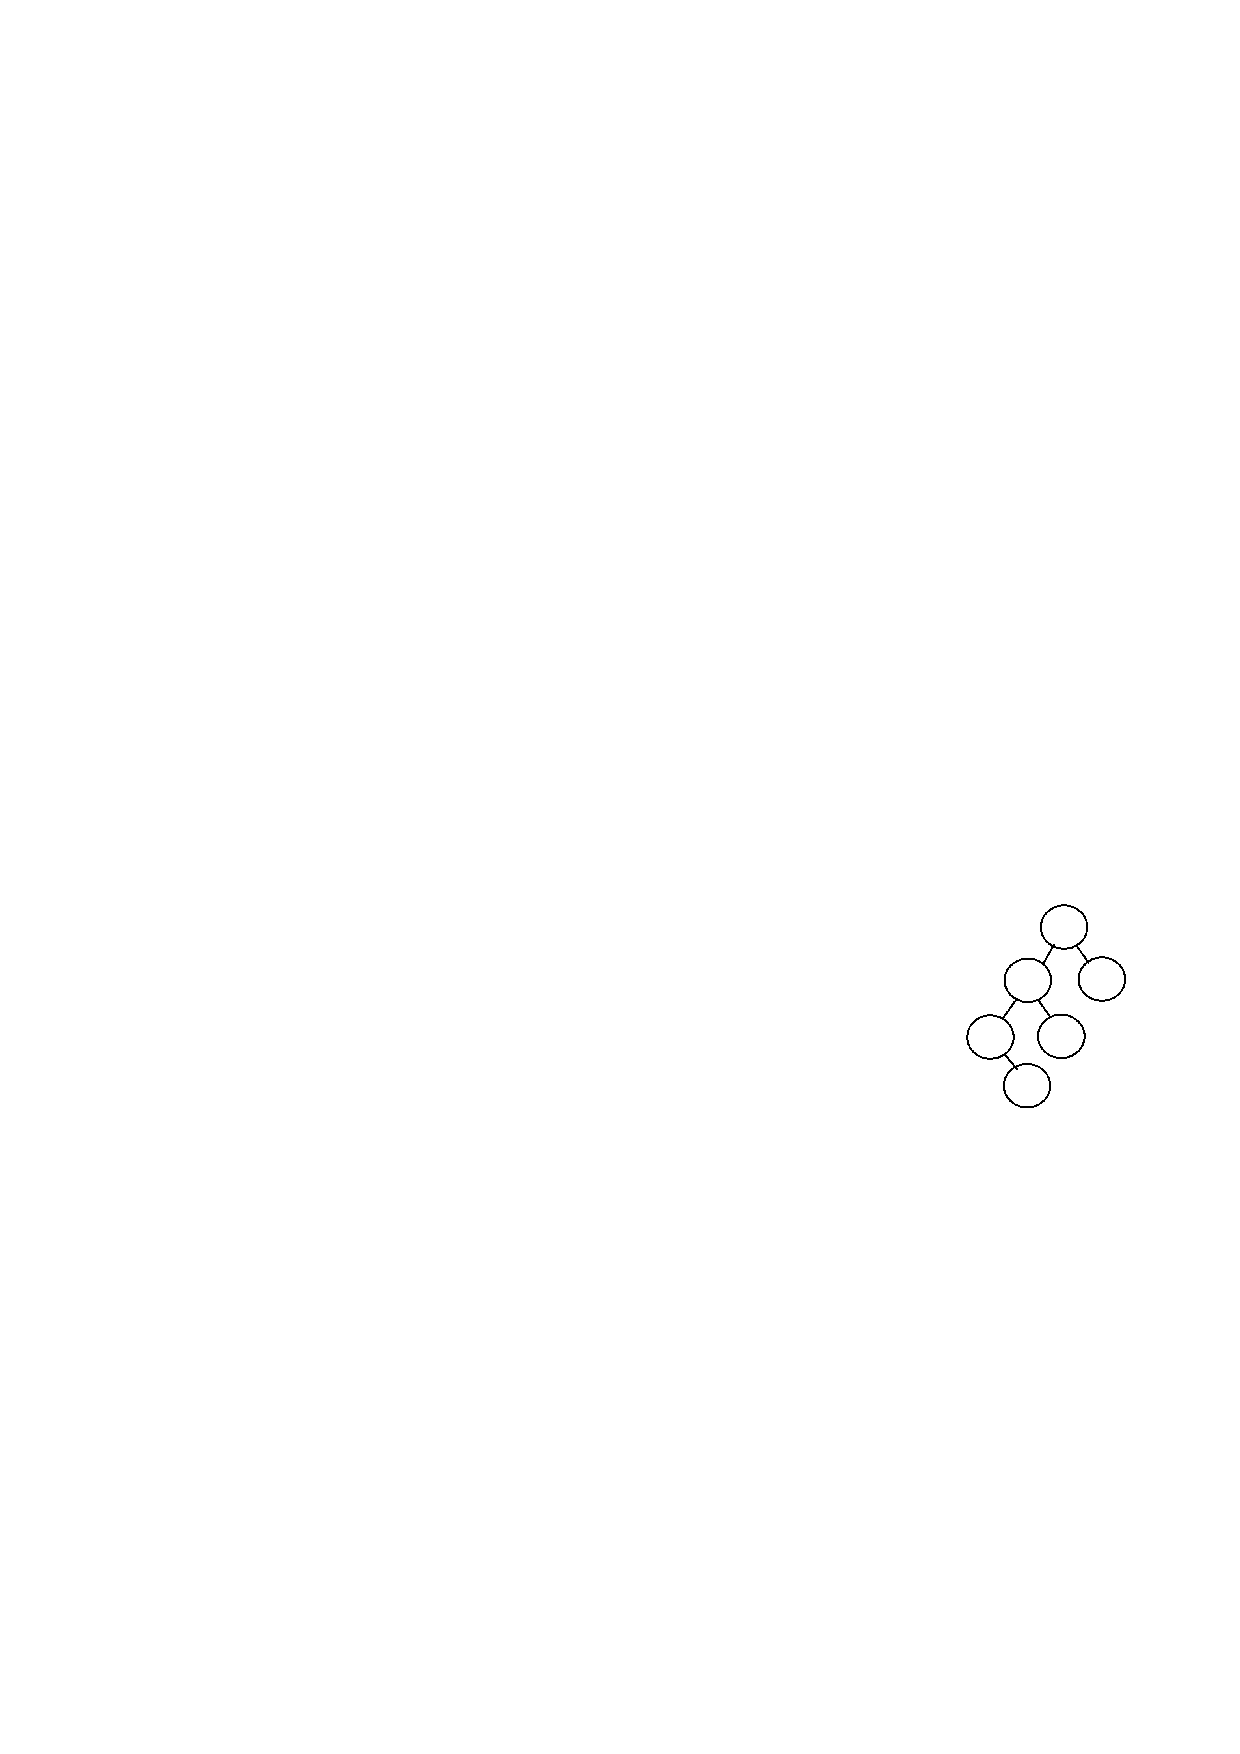
\includegraphics[width=.65\linewidth,height=.4\textheight,keepaspectratio]{../assets/figures/2023-questions-p001-b010.pdf}\end{center}

6．已知无向连通图G 中各边的权值均为1，下列算法中，一定能够求出图G 中从某顶点到其余各顶点最短路径的是\_\_\_\_\_\_。 I. 普里姆（Prim）算法 II. 克鲁斯卡尔（Kruskal）算法 III. 图的广度优先搜索算法


\begin{center}\begin{tabular}{>{\raggedright\arraybackslash}p{\dimexpr(\linewidth-8\tabcolsep)/4\relax}>{\raggedright\arraybackslash}p{\dimexpr(\linewidth-8\tabcolsep)/4\relax}>{\raggedright\arraybackslash}p{\dimexpr(\linewidth-8\tabcolsep)/4\relax}>{\raggedright\arraybackslash}p{\dimexpr(\linewidth-8\tabcolsep)/4\relax}}
\textbf{A.} 仅I & \textbf{B.} 仅III & \textbf{C.} 仅I、II & \textbf{D.} I、II、III\\[.35em]\end{tabular}\end{center}

7．下列关于非空B 树的叙述中，正确的是\_\_\_\_\_\_。 I. 插入操作可能增加树的高度 II. 删除操作一定会导致叶结点的变化 III. 查找某关键字总是要查找到叶结点 IV. 插入的新关键字最终位于叶结点中


\begin{center}\begin{tabular}{>{\raggedright\arraybackslash}p{\dimexpr(\linewidth-8\tabcolsep)/4\relax}>{\raggedright\arraybackslash}p{\dimexpr(\linewidth-8\tabcolsep)/4\relax}>{\raggedright\arraybackslash}p{\dimexpr(\linewidth-8\tabcolsep)/4\relax}>{\raggedright\arraybackslash}p{\dimexpr(\linewidth-8\tabcolsep)/4\relax}}
\textbf{A.} 仅I & \textbf{B.} 仅I、II & \textbf{C.} 仅III、IV & \textbf{D.} 仅I、II、IV\\[.35em]\end{tabular}\end{center}

8．对含有600 个元素的有序顺序表进行折半查找，关键字间的比较次数最多是\_\_\_\_\_\_。


\begin{center}\begin{tabular}{>{\raggedright\arraybackslash}p{\dimexpr(\linewidth-8\tabcolsep)/4\relax}>{\raggedright\arraybackslash}p{\dimexpr(\linewidth-8\tabcolsep)/4\relax}>{\raggedright\arraybackslash}p{\dimexpr(\linewidth-8\tabcolsep)/4\relax}>{\raggedright\arraybackslash}p{\dimexpr(\linewidth-8\tabcolsep)/4\relax}}
\textbf{A.} 9 & \textbf{B.} 10 & \textbf{C.} 30 & \textbf{D.} 300\\[.35em]\end{tabular}\end{center}

9．现有长度为5、初始为空的散列表HT，散列表函数\(\displaystyle H(k)=(k+4)\bmod 5\)，用线性探查再散列法解决冲突。若将关键字序列2022, 12, 25 依次插入HT 中，然后删除关键字25，则HT 中查找失败的平均查找长度为\_\_\_\_\_\_。


\begin{center}\begin{tabular}{>{\raggedright\arraybackslash}p{\dimexpr(\linewidth-8\tabcolsep)/4\relax}>{\raggedright\arraybackslash}p{\dimexpr(\linewidth-8\tabcolsep)/4\relax}>{\raggedright\arraybackslash}p{\dimexpr(\linewidth-8\tabcolsep)/4\relax}>{\raggedright\arraybackslash}p{\dimexpr(\linewidth-8\tabcolsep)/4\relax}}
\textbf{A.} 1 & \textbf{B.} 1.\allowbreak{}6 & \textbf{C.} 1.\allowbreak{}8 & \textbf{D.} 2.\allowbreak{}2\\[.35em]\end{tabular}\end{center}

10．下列排序算法中，不稳定的是\_\_\_\_\_\_。 I. 希尔排序 II. 归并排序 III. 快速排序 IV.堆排序 V. 基数排序


\begin{center}\begin{tabular}{>{\raggedright\arraybackslash}p{\dimexpr(\linewidth-8\tabcolsep)/4\relax}>{\raggedright\arraybackslash}p{\dimexpr(\linewidth-8\tabcolsep)/4\relax}>{\raggedright\arraybackslash}p{\dimexpr(\linewidth-8\tabcolsep)/4\relax}>{\raggedright\arraybackslash}p{\dimexpr(\linewidth-8\tabcolsep)/4\relax}}
\textbf{A.} I、II & \textbf{B.} II、V & \textbf{C.} I、III、IV & \textbf{D.} III、IV、V\\[.35em]\end{tabular}\end{center}

11．使用快速排序算法对数据进行升序排序，若经过一次划分后得到的数据序列是68, 11, 70, 23, 80,


第11题（续）：77, 48, 81, 93, 88，则该次划分的枢轴是\_\_\_\_\_\_。


\begin{center}\begin{tabular}{>{\raggedright\arraybackslash}p{\dimexpr(\linewidth-8\tabcolsep)/4\relax}>{\raggedright\arraybackslash}p{\dimexpr(\linewidth-8\tabcolsep)/4\relax}>{\raggedright\arraybackslash}p{\dimexpr(\linewidth-8\tabcolsep)/4\relax}>{\raggedright\arraybackslash}p{\dimexpr(\linewidth-8\tabcolsep)/4\relax}}
\textbf{A.} 11 & \textbf{B.} 70 & \textbf{C.} 80 & \textbf{D.} 81\\[.35em]\end{tabular}\end{center}

12．若机器M的主频为1.5GHz，在M上执行程序P的指令条数为\(\displaystyle 5\times10^5\)，P的平均CPI为1.2，则P在M上的指令执行速度和用户CPU时间分别为\_\_\_\_\_\_。


\begin{center}\begin{tabular}{>{\raggedright\arraybackslash}p{\dimexpr(\linewidth-4\tabcolsep)/2\relax}>{\raggedright\arraybackslash}p{\dimexpr(\linewidth-4\tabcolsep)/2\relax}}
\textbf{A.} 0.\allowbreak{}8GIPS，0.\allowbreak{}4ms & \textbf{B.} 0.\allowbreak{}8GIPS，\(\displaystyle 0.4\,\mu\mathrm{s}\)\\[.35em]
\textbf{C.} 1.\allowbreak{}25GIPS，0.\allowbreak{}4ms & \textbf{D.} 1.\allowbreak{}25GIPS，\(\displaystyle 0.4\,\mu\mathrm{s}\)\\[.35em]\end{tabular}\end{center}

13．若short 型变量x = -8 190，则x 的机器数是\_\_\_\_\_\_。


\begin{center}\begin{tabular}{>{\raggedright\arraybackslash}p{\dimexpr(\linewidth-8\tabcolsep)/4\relax}>{\raggedright\arraybackslash}p{\dimexpr(\linewidth-8\tabcolsep)/4\relax}>{\raggedright\arraybackslash}p{\dimexpr(\linewidth-8\tabcolsep)/4\relax}>{\raggedright\arraybackslash}p{\dimexpr(\linewidth-8\tabcolsep)/4\relax}}
\textbf{A.} E002H & \textbf{B.} E001H & \textbf{C.} 9FFFH & \textbf{D.} 9FFEH\\[.35em]\end{tabular}\end{center}

14．已知float型变量用IEEE 754单精度浮点数格式表示。若float型变量\(\displaystyle x\)的机器数为8020 0000H，则\(\displaystyle x\)的值是\_\_\_\_\_\_。


\begin{center}\begin{tabular}{>{\raggedright\arraybackslash}p{\dimexpr(\linewidth-8\tabcolsep)/4\relax}>{\raggedright\arraybackslash}p{\dimexpr(\linewidth-8\tabcolsep)/4\relax}>{\raggedright\arraybackslash}p{\dimexpr(\linewidth-8\tabcolsep)/4\relax}>{\raggedright\arraybackslash}p{\dimexpr(\linewidth-8\tabcolsep)/4\relax}}
\textbf{A.} \(\displaystyle -2^{-128}\) & \textbf{B.} \(\displaystyle -1.01\times2^{-127}\) & \textbf{C.} \(\displaystyle -1.01\times2^{-126}\) & \textbf{D.} 非数（NAN）\\[.35em]\end{tabular}\end{center}

15．某计算机的CPU 有30 根地址线，按字节编址，CPU 和主存芯片连接时，要求主存芯片占满所有可能存储地址空间，并且RAM 区和ROM 区所分配的空间大小比为3:1。若RAM 在连续低地址区，ROM 在连续高地址区，则ROM的地址范围\_\_\_\_\_\_。


\begin{center}\begin{tabular}{>{\raggedright\arraybackslash}p{\dimexpr(\linewidth-4\tabcolsep)/2\relax}>{\raggedright\arraybackslash}p{\dimexpr(\linewidth-4\tabcolsep)/2\relax}}
\textbf{A.} 0000 0000H～0FFF FFFFH & \textbf{B.} 1000 0000H～2FFF FFFFH\\[.35em]
\textbf{C.} 3000 0000H～3FFF FFFFH & \textbf{D.} 4000 0000H～4FFF FFFFH\\[.35em]\end{tabular}\end{center}

16．己知x、y 为int 类型，当x=100、y=200 时，执行“x 减y”指令得到的溢出标志OF 和借位标志 CF 分别为0、1，那么当x=10，y=–20 时，执行该指令得到的OF 和CF 分别是\_\_\_\_\_\_。


\begin{center}\begin{tabular}{>{\raggedright\arraybackslash}p{\dimexpr(\linewidth-8\tabcolsep)/4\relax}>{\raggedright\arraybackslash}p{\dimexpr(\linewidth-8\tabcolsep)/4\relax}>{\raggedright\arraybackslash}p{\dimexpr(\linewidth-8\tabcolsep)/4\relax}>{\raggedright\arraybackslash}p{\dimexpr(\linewidth-8\tabcolsep)/4\relax}}
\textbf{A.} OF=0，CF=0 & \textbf{B.} OF=0，CF=1 & \textbf{C.} OF=1，CF=0 & \textbf{D.} OF=1，CF=1\\[.35em]\end{tabular}\end{center}

17．某运算类型指令中有一个地址码为通用寄存器编号，对应通用寄存器中存放的是操作数或操作数的地址，CPU 区分两者的依据是\_\_\_\_\_\_。


\begin{center}\begin{tabular}{>{\raggedright\arraybackslash}p{\dimexpr(\linewidth-8\tabcolsep)/4\relax}>{\raggedright\arraybackslash}p{\dimexpr(\linewidth-8\tabcolsep)/4\relax}>{\raggedright\arraybackslash}p{\dimexpr(\linewidth-8\tabcolsep)/4\relax}>{\raggedright\arraybackslash}p{\dimexpr(\linewidth-8\tabcolsep)/4\relax}}
\textbf{A.} 操作数的寻址方式 & \textbf{B.} 操作数的编码方式 & \textbf{C.} 通用寄存器的编号 & \textbf{D.} 通用寄存器的内容\\[.35em]\end{tabular}\end{center}

18．数据通路由组合逻辑元件（操作元件）和时序逻辑元件组成（状态元件）组成，以下给出的元件中，属于操作元件的是\_\_\_\_\_\_。 I. 算术逻辑部件（ALU） II. 程序计数器（PC） III. 通用寄存器组（GPRs） IV. 多路选择器（MUX）


\begin{center}\begin{tabular}{>{\raggedright\arraybackslash}p{\dimexpr(\linewidth-8\tabcolsep)/4\relax}>{\raggedright\arraybackslash}p{\dimexpr(\linewidth-8\tabcolsep)/4\relax}>{\raggedright\arraybackslash}p{\dimexpr(\linewidth-8\tabcolsep)/4\relax}>{\raggedright\arraybackslash}p{\dimexpr(\linewidth-8\tabcolsep)/4\relax}}
\textbf{A.} 仅I、II & \textbf{B.} 仅I、IV & \textbf{C.} 仅II、III & \textbf{D.} 仅I、II、IV\\[.35em]\end{tabular}\end{center}

19．某系统采用“取指、译码/取数、执行、访存、写回”5段流水线，RISC处理器中执行如下指令序列（第一列为指令序号），其中s0、s1、s2、s3、t2表示寄存器编号。


\begin{Verbatim}[breaklines,breakanywhere,fontsize=\small]
I1  add s2, s1, s0    // R[s2]←R[s1]+R[s0]
I2  load s3, 0(s2)    // R[s3]←M[R[s2]+0]
I3  beq t2, s3, L1    // if R[t2]=R[s3] jump to L1
I4  addi t2, t2, 20   // R[t2]←R[t2]+20
I5  L1:...
\end{Verbatim}

若采用转发（旁路）技术处理数据冒险，采用硬件阻塞方式处理控制冒险，则在I1～I4执行过程中，发生流水线阻塞的指令有\_\_\_\_\_\_。


\begin{center}\begin{tabular}{>{\raggedright\arraybackslash}p{\dimexpr(\linewidth-8\tabcolsep)/4\relax}>{\raggedright\arraybackslash}p{\dimexpr(\linewidth-8\tabcolsep)/4\relax}>{\raggedright\arraybackslash}p{\dimexpr(\linewidth-8\tabcolsep)/4\relax}>{\raggedright\arraybackslash}p{\dimexpr(\linewidth-8\tabcolsep)/4\relax}}
\textbf{A.} 仅I3 & \textbf{B.} 仅I2、I4 & \textbf{C.} 仅I3、I4 & \textbf{D.} I2、I3、I4\\[.35em]\end{tabular}\end{center}

20．某存储总线宽度为64b，总线时钟频率为1GHz，在总线上传输一个数据或地址需要一个时钟周期， 不支持突发传送方式。若通过该总线连接CPU 和主存，主存每次准备一个64b 数据需要6ns，主存块大小为32B，则读取一个主存块需要的时间是\_\_\_\_\_\_。


\begin{center}\begin{tabular}{>{\raggedright\arraybackslash}p{\dimexpr(\linewidth-8\tabcolsep)/4\relax}>{\raggedright\arraybackslash}p{\dimexpr(\linewidth-8\tabcolsep)/4\relax}>{\raggedright\arraybackslash}p{\dimexpr(\linewidth-8\tabcolsep)/4\relax}>{\raggedright\arraybackslash}p{\dimexpr(\linewidth-8\tabcolsep)/4\relax}}
\textbf{A.} 8ns & \textbf{B.} 11ns & \textbf{C.} 26ns & \textbf{D.} 32ns\\[.35em]\end{tabular}\end{center}

21．下列关于硬件和异常/中断关系的叙述中，错误的是（\_\_\_\_\_\_）。


\begin{center}\begin{tabular}{>{\raggedright\arraybackslash}p{\dimexpr(\linewidth-4\tabcolsep)/2\relax}>{\raggedright\arraybackslash}p{\dimexpr(\linewidth-4\tabcolsep)/2\relax}}
\textbf{A.} CPU 在执行一条指令过程中检测异常事件 & \textbf{B.} CPU 在执行完一条指令时检测中断请求信号\\[.35em]
\textbf{C.} 开中断时CPU 检测到中断请求后就进行中断响应 & \textbf{D.} 外部设备通过中断控制器向CPU 发中断结束信号\\[.35em]\end{tabular}\end{center}

22．下列关于I/O 控制方式的叙述中，错误的是\_\_\_\_\_\_。


\begin{center}\begin{tabular}{>{\raggedright\arraybackslash}p{\dimexpr(\linewidth-4\tabcolsep)/2\relax}>{\raggedright\arraybackslash}p{\dimexpr(\linewidth-4\tabcolsep)/2\relax}}
\textbf{A.} 查询方式下，通过CPU 执行查询程序进行I/O 操作 & \\[.35em]\end{tabular}\end{center}

第22题（续）：


\begin{center}\begin{tabular}{>{\raggedright\arraybackslash}p{\dimexpr(\linewidth-4\tabcolsep)/2\relax}>{\raggedright\arraybackslash}p{\dimexpr(\linewidth-4\tabcolsep)/2\relax}}
\textbf{B.} 中断方式下，通过CPU 执行中断服务程序进行I/O 操作 & \textbf{C.} DMA 方式下，通过CPU 执行DMA 传送程序进行I/O 操作\\[.35em]
\textbf{D.} 对于SSD、网络适配器等高速设备，采用DMA 方式输入/输出 & \\[.35em]\end{tabular}\end{center}

23．与宏内核操作系统相比，下列特征中，微内核操作系统具有的是\_\_\_\_\_\_。 I. 较好的性能 II. 较高的可靠性 III. 较高的安全性 IV. 较强的可扩展性


\begin{center}\begin{tabular}{>{\raggedright\arraybackslash}p{\dimexpr(\linewidth-8\tabcolsep)/4\relax}>{\raggedright\arraybackslash}p{\dimexpr(\linewidth-8\tabcolsep)/4\relax}>{\raggedright\arraybackslash}p{\dimexpr(\linewidth-8\tabcolsep)/4\relax}>{\raggedright\arraybackslash}p{\dimexpr(\linewidth-8\tabcolsep)/4\relax}}
\textbf{A.} 仅II、IV & \textbf{B.} 仅I、II、III & \textbf{C.} 仅I、III、IV & \textbf{D.} 仅II、III、IV\\[.35em]\end{tabular}\end{center}

24．在操作系统内核中，中断向量表适合采用的数据结构是\_\_\_\_\_\_。


\begin{center}\begin{tabular}{>{\raggedright\arraybackslash}p{\dimexpr(\linewidth-8\tabcolsep)/4\relax}>{\raggedright\arraybackslash}p{\dimexpr(\linewidth-8\tabcolsep)/4\relax}>{\raggedright\arraybackslash}p{\dimexpr(\linewidth-8\tabcolsep)/4\relax}>{\raggedright\arraybackslash}p{\dimexpr(\linewidth-8\tabcolsep)/4\relax}}
\textbf{A.} 数组 & \textbf{B.} 队列 & \textbf{C.} 单向链表 & \textbf{D.} 双向链表\\[.35em]\end{tabular}\end{center}

25．某系统采用页式存储管理，用位图管理空闲页框。若页大小为4KB，物理内存大小为16GB，则位图所占空间的大小是\_\_\_\_\_\_。


\begin{center}\begin{tabular}{>{\raggedright\arraybackslash}p{\dimexpr(\linewidth-8\tabcolsep)/4\relax}>{\raggedright\arraybackslash}p{\dimexpr(\linewidth-8\tabcolsep)/4\relax}>{\raggedright\arraybackslash}p{\dimexpr(\linewidth-8\tabcolsep)/4\relax}>{\raggedright\arraybackslash}p{\dimexpr(\linewidth-8\tabcolsep)/4\relax}}
\textbf{A.} 128B & \textbf{B.} 128KB & \textbf{C.} 512KB & \textbf{D.} 4MB\\[.35em]\end{tabular}\end{center}

26．下列操作完成时，导致CPU 从内核态转为用户态的是\_\_\_\_\_\_。


\begin{center}\begin{tabular}{>{\raggedright\arraybackslash}p{\dimexpr(\linewidth-8\tabcolsep)/4\relax}>{\raggedright\arraybackslash}p{\dimexpr(\linewidth-8\tabcolsep)/4\relax}>{\raggedright\arraybackslash}p{\dimexpr(\linewidth-8\tabcolsep)/4\relax}>{\raggedright\arraybackslash}p{\dimexpr(\linewidth-8\tabcolsep)/4\relax}}
\textbf{A.} 阻塞进程 & \textbf{B.} 执行CPU 调度 & \textbf{C.} 唤醒进程 & \textbf{D.} 执行系统调用\\[.35em]\end{tabular}\end{center}

27．下列由当前线程引起的事件或执行的操作中，可能导致该线程由执行形态变为就绪态的是\_\_\_\_\_\_。


\begin{center}\begin{tabular}{>{\raggedright\arraybackslash}p{\dimexpr(\linewidth-4\tabcolsep)/2\relax}>{\raggedright\arraybackslash}p{\dimexpr(\linewidth-4\tabcolsep)/2\relax}}
\textbf{A.} 键盘输入 & \textbf{B.} 缺页异常\\[.35em]
\textbf{C.} 主动出让CPU & \textbf{D.} 执行信号量的wait()操作\\[.35em]\end{tabular}\end{center}

28．对于采用虚拟内存管理方式的系统，下列关于进程虚拟地址空间的叙述中，错误的是\_\_\_\_\_\_。


\begin{center}\begin{tabular}{>{\raggedright\arraybackslash}p{\dimexpr(\linewidth-4\tabcolsep)/2\relax}>{\raggedright\arraybackslash}p{\dimexpr(\linewidth-4\tabcolsep)/2\relax}}
\textbf{A.} 每个进程都有自已独立的虚拟地址空间 & \textbf{B.} C 语言中malloc()函数返回的是虚拟地址\\[.35em]
\textbf{C.} 进程对数据段和代码段可以有不同的访问权限 & \textbf{D.} 虚拟地址空间的大小由内存和硬盘的大小决定\\[.35em]\end{tabular}\end{center}

29．进程P1、P2和P3进入就绪队列的时刻、优先级（值越大优先权越高）以及CPU的执行时间如下表所示。


\begin{center}\begin{adjustbox}{max width=\linewidth}\begin{tabular}{|>{\raggedright\arraybackslash}p{\dimexpr(\linewidth-8\tabcolsep-5\arrayrulewidth)/4\relax}|>{\raggedright\arraybackslash}p{\dimexpr(\linewidth-8\tabcolsep-5\arrayrulewidth)/4\relax}|>{\raggedright\arraybackslash}p{\dimexpr(\linewidth-8\tabcolsep-5\arrayrulewidth)/4\relax}|>{\raggedright\arraybackslash}p{\dimexpr(\linewidth-8\tabcolsep-5\arrayrulewidth)/4\relax}|}\hline
进程名 & 进入就绪队列的时刻 & 优先数 & CPU执行时间\\\hline
P1 & 0ms & 1 & 60ms\\\hline
P2 & 20ms & 10 & 42ms\\\hline
P3 & 30ms & 100 & 13ms\\\hline\end{tabular}\end{adjustbox}\end{center}

若系统采用基于优先权的抢占式CPU调度算法，从0ms时刻开始进行调度，则P1、P2和P3的平均周转时间为\_\_\_\_\_\_。


\begin{center}\begin{tabular}{>{\raggedright\arraybackslash}p{\dimexpr(\linewidth-8\tabcolsep)/4\relax}>{\raggedright\arraybackslash}p{\dimexpr(\linewidth-8\tabcolsep)/4\relax}>{\raggedright\arraybackslash}p{\dimexpr(\linewidth-8\tabcolsep)/4\relax}>{\raggedright\arraybackslash}p{\dimexpr(\linewidth-8\tabcolsep)/4\relax}}
\textbf{A.} 60ms & \textbf{B.} 61ms & \textbf{C.} 70ms & \textbf{D.} 71ms\\[.35em]\end{tabular}\end{center}

30．进程R 和S 共享数据data，若data 在R 和S 中所在页的页号分别为p1 和p2，两个页所对应的页框号分别为f1 和f2，则下列叙述中，正确的是\_\_\_\_\_\_。


\begin{center}\begin{tabular}{>{\raggedright\arraybackslash}p{\dimexpr(\linewidth-4\tabcolsep)/2\relax}>{\raggedright\arraybackslash}p{\dimexpr(\linewidth-4\tabcolsep)/2\relax}}
\textbf{A.} p1 和p2 一定相等，f1 和f2 一定相等 & \textbf{B.} p1 和p2 一定相等，f1 和f2 不一定相等\\[.35em]
\textbf{C.} p1 和p2 不一定相等，f1 和f2 一定相等 & \textbf{D.} p1 和p2 不一定相等，f1 和f2 不一定相等\\[.35em]\end{tabular}\end{center}

31．若文件F 仅被进程P 打开并访问，则当进程P 关闭F 时，下列操作中，文件系统需要完成的是\_\_\_\_\_\_。


\begin{center}\begin{tabular}{>{\raggedright\arraybackslash}p{\dimexpr(\linewidth-4\tabcolsep)/2\relax}>{\raggedright\arraybackslash}p{\dimexpr(\linewidth-4\tabcolsep)/2\relax}}
\textbf{A.} 删除目录文件中F 的目录项 & \textbf{B.} 释放F 的索引节点所占的内存空间\\[.35em]
\textbf{C.} 释放F 的索引节点所占的外存空间 & \textbf{D.} 将文件磁盘索引结点中的链接计数减1\\[.35em]\end{tabular}\end{center}

32．下列因素中，设备分配需要考虑的是\_\_\_\_\_\_。 I.设备的类型 II. 设备的访问权限 III.设备的占用状态 IV. 逻辑设备与物理设备的映射关系


\begin{center}\begin{tabular}{>{\raggedright\arraybackslash}p{\dimexpr(\linewidth-8\tabcolsep)/4\relax}>{\raggedright\arraybackslash}p{\dimexpr(\linewidth-8\tabcolsep)/4\relax}>{\raggedright\arraybackslash}p{\dimexpr(\linewidth-8\tabcolsep)/4\relax}>{\raggedright\arraybackslash}p{\dimexpr(\linewidth-8\tabcolsep)/4\relax}}
\textbf{A.} 仅I、II & \textbf{B.} 仅II、III & \textbf{C.} 仅III、IV & \textbf{D.} I、II、III、IV\\[.35em]\end{tabular}\end{center}

33．在下图所示的分组交换网络中，主机H1 和H2 通过路由器互连，2 段链路的带宽均为100Mb/s、 时延带宽积（即单向传播时延×宽带）均为1000b。若H1 向H2 发送1 个大小为1MB 的文件， 分组长度为1000B，则从H1 开始发送时刻起到H2 收到文件全部数据时刻止，所需的时间至少是 \_\_\_\_\_\_（注：\(\displaystyle \mathrm{M}=10^6\)）。


第33题（续）：


\begin{center}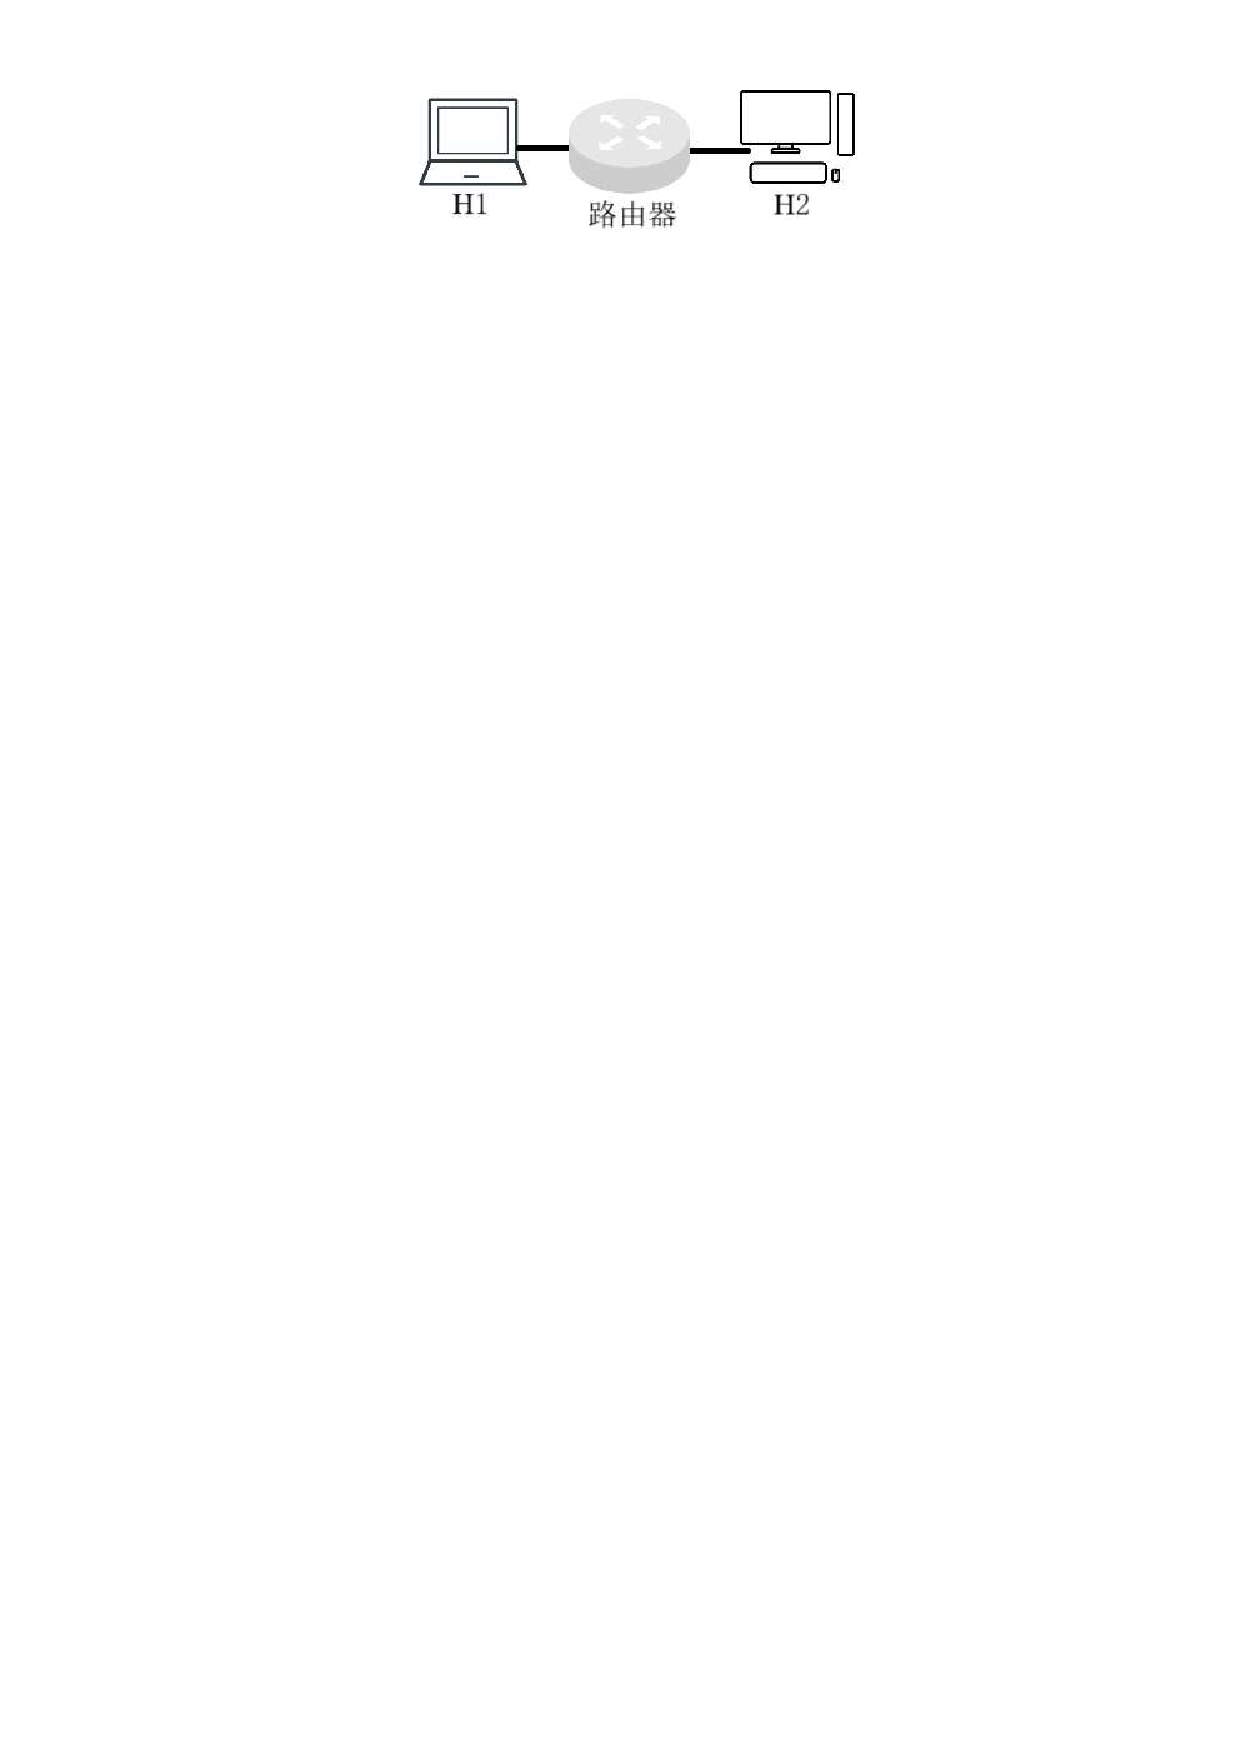
\includegraphics[width=.65\linewidth,height=.4\textheight,keepaspectratio]{../assets/figures/2023-questions-p004-b001.pdf}\end{center}

\begin{center}\begin{tabular}{>{\raggedright\arraybackslash}p{\dimexpr(\linewidth-8\tabcolsep)/4\relax}>{\raggedright\arraybackslash}p{\dimexpr(\linewidth-8\tabcolsep)/4\relax}>{\raggedright\arraybackslash}p{\dimexpr(\linewidth-8\tabcolsep)/4\relax}>{\raggedright\arraybackslash}p{\dimexpr(\linewidth-8\tabcolsep)/4\relax}}
\textbf{A.} 80.\allowbreak{}02ms & \textbf{B.} 80.\allowbreak{}08ms & \textbf{C.} 80.\allowbreak{}09ms & \textbf{D.} 80.\allowbreak{}10ms\\[.35em]\end{tabular}\end{center}

34．某无噪声理想信道带宽为4MHz，采用QAM 调制，若该信道的最大数据传输速率是48Mb/s，则该信道采用的QAM 调制方案是\_\_\_\_\_\_。


\begin{center}\begin{tabular}{>{\raggedright\arraybackslash}p{\dimexpr(\linewidth-8\tabcolsep)/4\relax}>{\raggedright\arraybackslash}p{\dimexpr(\linewidth-8\tabcolsep)/4\relax}>{\raggedright\arraybackslash}p{\dimexpr(\linewidth-8\tabcolsep)/4\relax}>{\raggedright\arraybackslash}p{\dimexpr(\linewidth-8\tabcolsep)/4\relax}}
\textbf{A.} QAM–16 & \textbf{B.} QAM–32 & \textbf{C.} QAM–64 & \textbf{D.} QAM–128\\[.35em]\end{tabular}\end{center}

35．假设通过同一信道，数据链路层分别采用停止–等待协议、GBN 协议和SR 协议（发送窗口和接收窗口相等）传输数据，3 个协议数据帧长相同，忽略确认帧长度，帧序号位数为3 比特。若对应 3 个协议的发送方最大信道利用率分别是U1、\(\displaystyle U_2\) 和U3，则U1、\(\displaystyle U_2\) 和U3 满足的关系是\_\_\_\_\_\_。


\begin{center}\begin{tabular}{>{\raggedright\arraybackslash}p{\dimexpr(\linewidth-4\tabcolsep)/2\relax}>{\raggedright\arraybackslash}p{\dimexpr(\linewidth-4\tabcolsep)/2\relax}}
\textbf{A.} \(\displaystyle U_1\)≤\(\displaystyle U_2\)≤\(\displaystyle U_3\) & \textbf{B.} \(\displaystyle U_1\)≤\(\displaystyle U_3\)≤\(\displaystyle U_2\)\\[.35em]
\textbf{C.} \(\displaystyle U_2\)≤\(\displaystyle U_3\)≤\(\displaystyle U_1\) & \textbf{D.} \(\displaystyle U_3\)≤\(\displaystyle U_2\)≤\(\displaystyle U_1\)\\[.35em]\end{tabular}\end{center}

36．已知10BaseT 以太网的争用时间片为\(\displaystyle 51.2\,\mu\mathrm{s}\)。若网卡在发送某帧时发生了连续4 次冲突，则基于二进制指数退避算法确定的再次尝试重发该帧前等待的最长时间是\_\_\_\_\_\_。


\begin{center}\begin{tabular}{>{\raggedright\arraybackslash}p{\dimexpr(\linewidth-8\tabcolsep)/4\relax}>{\raggedright\arraybackslash}p{\dimexpr(\linewidth-8\tabcolsep)/4\relax}>{\raggedright\arraybackslash}p{\dimexpr(\linewidth-8\tabcolsep)/4\relax}>{\raggedright\arraybackslash}p{\dimexpr(\linewidth-8\tabcolsep)/4\relax}}
\textbf{A.} \(\displaystyle 51.2\,\mu\mathrm{s}\) & \textbf{B.} \(\displaystyle 204.8\,\mu\mathrm{s}\) & \textbf{C.} \(\displaystyle 768\,\mu\mathrm{s}\) & \textbf{D.} \(\displaystyle 819.2\,\mu\mathrm{s}\)\\[.35em]\end{tabular}\end{center}

37．若甲向乙发送数据时采用CRC校验，生成多项式为\(\displaystyle G(X)=X^4+X+1\)（即G=10011），则乙接收到下列比特串时，可以断定其在传输过程中未发生错误的是\_\_\_\_\_\_。


\begin{center}\begin{tabular}{>{\raggedright\arraybackslash}p{\dimexpr(\linewidth-8\tabcolsep)/4\relax}>{\raggedright\arraybackslash}p{\dimexpr(\linewidth-8\tabcolsep)/4\relax}>{\raggedright\arraybackslash}p{\dimexpr(\linewidth-8\tabcolsep)/4\relax}>{\raggedright\arraybackslash}p{\dimexpr(\linewidth-8\tabcolsep)/4\relax}}
\textbf{A.} 1 0111 0000 & \textbf{B.} 1 0111 0100 & \textbf{C.} 1 0111 1000 & \textbf{D.} 1 0111 1100\\[.35em]\end{tabular}\end{center}

38．某网络拓扑如下图所示，其中路出器R2 实现NAT 功能。若主机H 向Internet 发送1 个IP 分组， 则经过R2 转发后，该IP 分组的源IP 地址是\_\_\_\_\_\_。


\begin{center}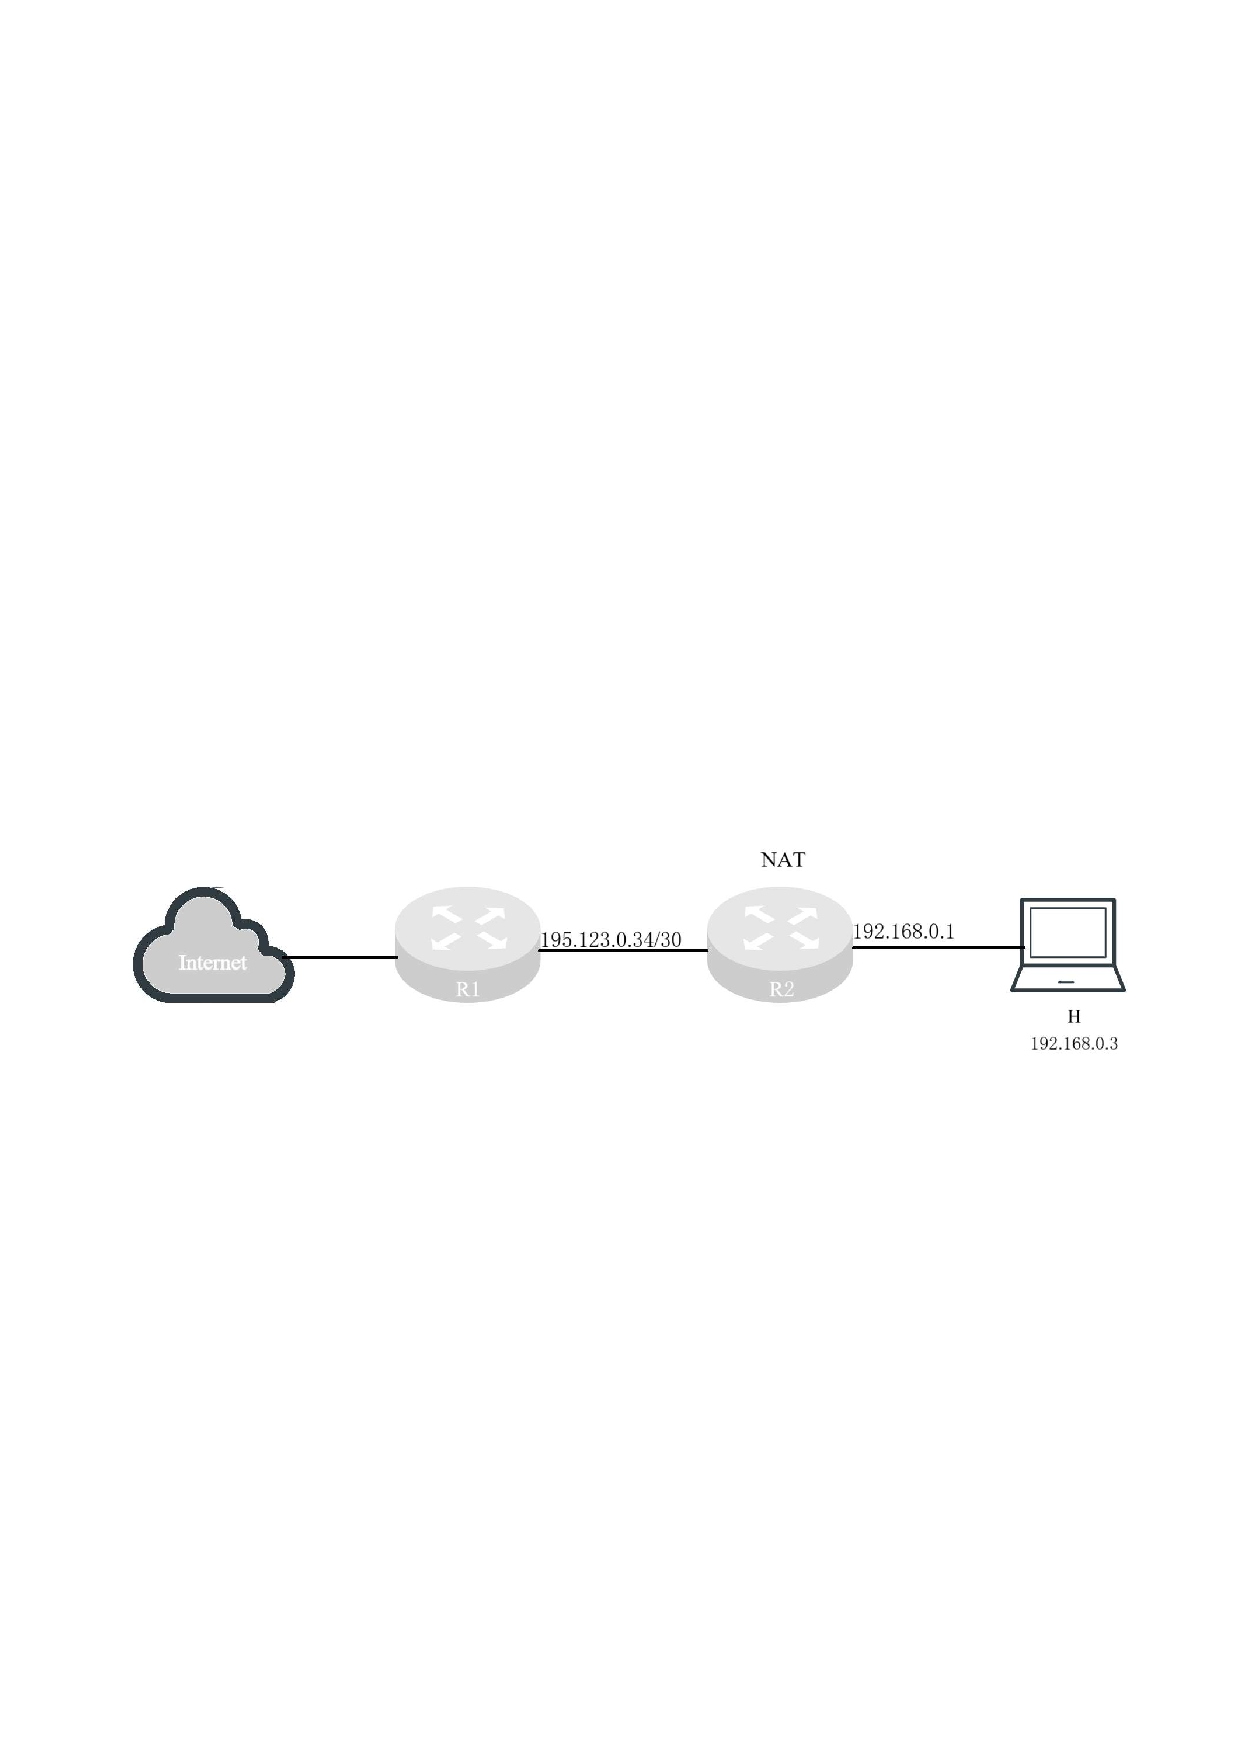
\includegraphics[width=.65\linewidth,height=.4\textheight,keepaspectratio]{../assets/figures/2023-questions-p004-b008.pdf}\end{center}

\begin{center}\begin{tabular}{>{\raggedright\arraybackslash}p{\dimexpr(\linewidth-8\tabcolsep)/4\relax}>{\raggedright\arraybackslash}p{\dimexpr(\linewidth-8\tabcolsep)/4\relax}>{\raggedright\arraybackslash}p{\dimexpr(\linewidth-8\tabcolsep)/4\relax}>{\raggedright\arraybackslash}p{\dimexpr(\linewidth-8\tabcolsep)/4\relax}}
\textbf{A.} 195.\allowbreak{}123.\allowbreak{}0.\allowbreak{}33 & \textbf{B.} 192.\allowbreak{}123.\allowbreak{}0.\allowbreak{}35 & \textbf{C.} 192.\allowbreak{}168.\allowbreak{}0.\allowbreak{}1 & \textbf{D.} 192.\allowbreak{}168.\allowbreak{}0.\allowbreak{}3\\[.35em]\end{tabular}\end{center}

39．主机168.16.84.24/20 所在子网的最小可分配IP 地址和最大可分配IP 地址分别是\_\_\_\_\_\_。


\begin{center}\begin{tabular}{>{\raggedright\arraybackslash}p{\dimexpr(\linewidth-4\tabcolsep)/2\relax}>{\raggedright\arraybackslash}p{\dimexpr(\linewidth-4\tabcolsep)/2\relax}}
\textbf{A.} 168.\allowbreak{}16.\allowbreak{}80.\allowbreak{}1, 168.\allowbreak{}16.\allowbreak{}84.\allowbreak{}254 & \textbf{B.} 168.\allowbreak{}16.\allowbreak{}80.\allowbreak{}1, 168.\allowbreak{}16.\allowbreak{}95.\allowbreak{}254\\[.35em]
\textbf{C.} 168.\allowbreak{}16.\allowbreak{}84.\allowbreak{}1, 168.\allowbreak{}16.\allowbreak{}84.\allowbreak{}254 & \textbf{D.} 168.\allowbreak{}16.\allowbreak{}84.\allowbreak{}1, 168.\allowbreak{}16.\allowbreak{}95.\allowbreak{}254\\[.35em]\end{tabular}\end{center}

40．下列关于IPv4 和IPv6 的叙述中，正确的是（\_\_\_\_\_\_）。 I. IPv6 地址空间是IPv4 地址空间的96 倍 II. IPv4 首部和IPv6 的基本首部的长度均可变 III. IPv4 向IPv6 过渡可以采用双协议栈和隧道技术 IV. IPv6 首部的Hop Limit 等价于IPv4 首部的TTL 字段


\begin{center}\begin{tabular}{>{\raggedright\arraybackslash}p{\dimexpr(\linewidth-8\tabcolsep)/4\relax}>{\raggedright\arraybackslash}p{\dimexpr(\linewidth-8\tabcolsep)/4\relax}>{\raggedright\arraybackslash}p{\dimexpr(\linewidth-8\tabcolsep)/4\relax}>{\raggedright\arraybackslash}p{\dimexpr(\linewidth-8\tabcolsep)/4\relax}}
\textbf{A.} 仅I、II & \textbf{B.} 仅I、IV & \textbf{C.} 仅II、III & \textbf{D.} 仅III、IV\\[.35em]\end{tabular}\end{center}

\subsection*{二、综合应用题（第41～47小题，共70分）}

41．（13分）已知有向图G采用邻接矩阵存储，类型定义如下：


\begin{Verbatim}[breaklines,breakanywhere,fontsize=\small]
typedef struct             // 图的类型定义
{
    int numVertices, numEdges;   // 图的顶点数和有向边数
    char VerticesList[MAXV];     // 顶点表，MAXV 为已定义常量
    int Edge[MAXV][MAXV];        // 邻接矩阵
}MGraph
\end{Verbatim}

\begin{center}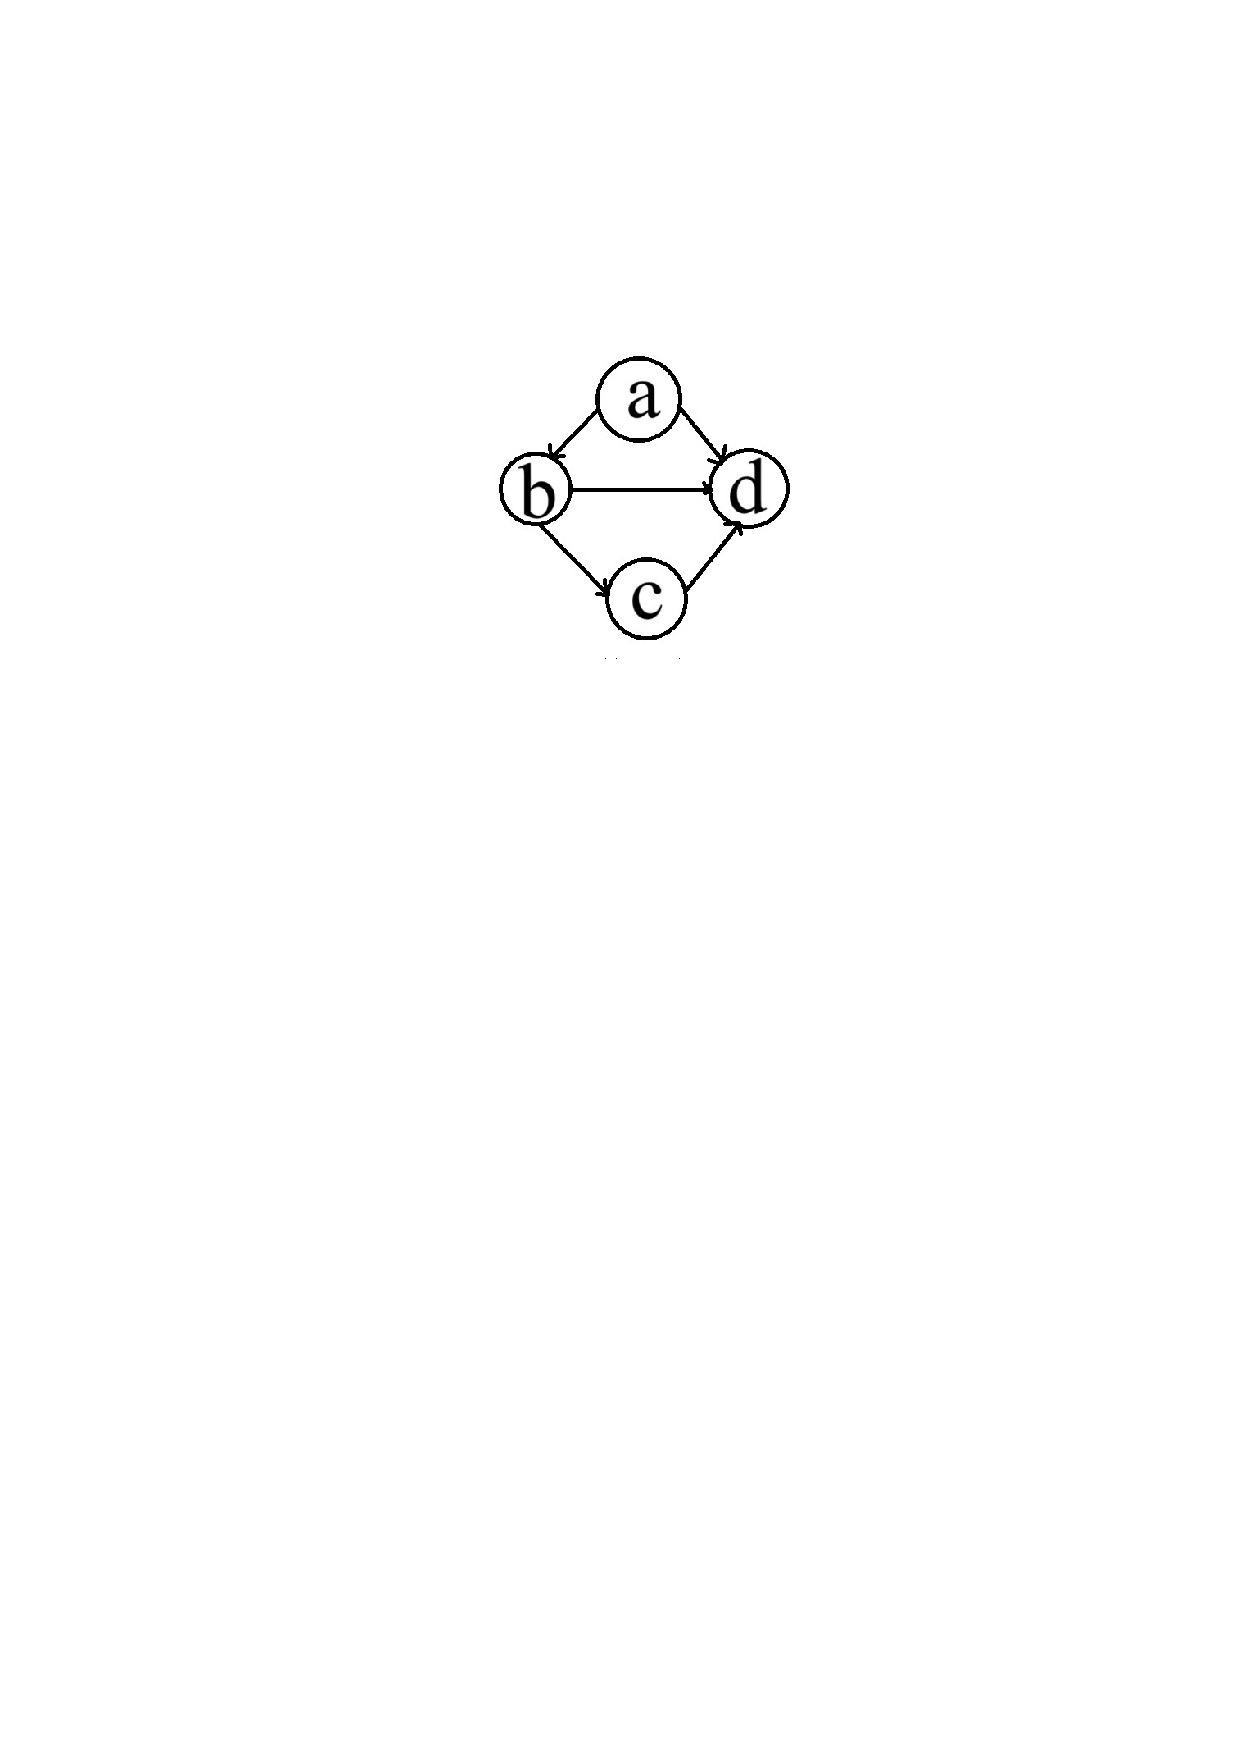
\includegraphics[width=.65\linewidth,height=.4\textheight,keepaspectratio]{../assets/figures/2023-questions-p005-b003.pdf}\end{center}

将图中出度大于入度的顶点称为K顶点。例如题41图中，顶点a和顶点b为K顶点。请设计算法：int printVertices(MGraph G)，对给定的任意非空有向图G，输出图G中所有的K顶点，并返回K顶点的个数。要求：（1）给出算法的基本设计思想。（2）根据设计思想，采用C或C++语言描述算法，关键之处给出注释。


42．（10分）对含有\(\displaystyle n\)（\(\displaystyle n>0\)）个记录的文件进行外部排序，采用置换-选择排序生成初始归并段时需要使用一个工作，工作区中能保存\(\displaystyle m\)个记录，请回答下列问题：（1）若文件中含有19个记录，其关键字依次是51, 94, 37, 92, 14, 63, 15, 99, 48, 56, 23, 60, 31, 17, 43, 8, 90, 166, 100，当\(\displaystyle m=4\)时，可生成几个初始归并段？各是什么？（2）对任意的\(\displaystyle m\)（\(\displaystyle n\gg m>0\)），生成的第一个初始归并段的长度最大值和最小值分别是多少？


43．（14分）已知计算机M字长为32位，按字节编址，采用请求调页策略的虚拟存储管理方式，虚拟地址32位，页面大小为4KB；数据Cache采用4路组相联映射方式，数据区大小为8KB，主存块大小为32B。现有C语言程序段如下：


\begin{Verbatim}[breaklines,breakanywhere,fontsize=\small]
int a[24][64];
...
for (i=0; i<24; i++)
    for (j=0; j<64; j++) a[i][j]=10;
\end{Verbatim}

已知二维数组a按行优先存放，在虚拟地址空间中分配的起始地址为0042 2000H，sizeof(int)=4。假定在M上执行上述程序段之前数组a不在主存，且在该程序执行过程中不会发生页面置换。请回答下列问题：（1）数组分布在几个页面中？对于数组a的访问，会发生几次缺页异常？页故障地址各是什么？（2）不考虑变量i和j，该程序段的数据访问是否具有时间局部性？为什么？（3）计算机M的虚拟地址(A31～A0)中哪几位用作块内地址？哪几位用作Cache组号？a[1][0]的虚拟地址是多少？其所在主存块对应的Cache组号是多少？（4）数组a占用多少主存块？假设上述程序段执行过程中数组a的访问不会和其他数据发生Cache访问冲突，则数组a的Cache命中率是多少？若将循环中i和j的次序按如下方式调换：


\begin{Verbatim}[breaklines,breakanywhere,fontsize=\small]
for (j=0; j<64; j++)
    for (i=0; i<24; i++) a[i][j]=10;
\end{Verbatim}

则数组a的Cache命中率又是多少？


44．（9分）第43题中C程序段在计算机M上的部分机器级代码如下，每个机器级代码行中依次包含指令序号、虚拟地址、机器指令和汇编指令。


\begin{Verbatim}[breaklines,breakanywhere,fontsize=\small]
for (i=0; i<24; i++)
1   00401072  C7 45 F8 00 00 00 00        mov [ebp–8], 0
2   00401079  EB 09                       jmp 00401084h
3   0040107B  8B 55 F8                    mov eax, [ebp–8]
    ...       ...                         ...
7   00401088  7D 32                       jge 004010BCh
for (j=0; j<64; j++)
8   0040108A  C7 45 FC 00 00 00 00        mov [ebp–4], 0
    ...       ...                         ...
a[i][j]=10;
    ...       ...                         ...
19  004010AE  C7 84 82 00 20 42 00 0A     mov [ecx + edx * 4+
               00 00 00                   00422000h], 0Ah
\end{Verbatim}

请回答下列问题：（1）第20条指令的虚拟地址是多少？（2）已知第2条jmp和第7条jge都是跳转指令，其操作码分别是EBH和7DH，跳转目标地址分别为0040 1084H、0040 10BCH，这两条指令分别采用什么寻址方式？请给出第2条指令jmp的跳转目标地址计算过程。（3）已知第19条mov指令的功能是“a[i][j]←10”，其中ecx和edx为寄存器名，0042 2000H是数组a的首地址，指令中源操作数采用什么寻址方式？已知edx中存放的是变量j，ecx中存放的是什么？根据该指令的机器码判断计算机M采用的是大端还是小端方式。（4）第1次执行第19条指令时，取指令过程中是否会发生缺页异常？为什么？


45．（7分）现要求学生使用swap指令和布尔型变量lock，实现临界区互斥。lock为线程间共享的变量。lock的值为TRUE时线程不能进入临界区，为FALSE时，线程能进入临界区。某同学编写的实现临界区互斥的伪代码如题45（a）图所示；题45（b）图给出newSwap()的代码。


题45（a）图　某同学写的伪代码：


\begin{Verbatim}[breaklines,breakanywhere,fontsize=\small]
bool lock=false;       // 共享变量
......
bool key=True          // 进入区
if(key == TRUE)
    swap key,lock;
// 临界区
lock=TRUE;             // 退出区
\end{Verbatim}

题45（b）图　newSwap()的代码：


\begin{Verbatim}[breaklines,breakanywhere,fontsize=\small]
void newSwap(bool*a, bool*b)
{
    bool temp=*a;
    *a=*b;
    *b=temp;
}
\end{Verbatim}

请回答下列问题：（1）题45（a）图的伪代码中哪些语句存在错误？将其改为正确的语句（不增加语句条数）。（2）题45（b）图给出了两个变量值的函数newSwap()的代码，是否可以用函数调用语句“newSwap(\&key，\&lock)”代替指令“swap key, lock”以实现临界区的互斥？为什么？


46．（8分）进程P通过执行系统调用从键盘接收一个字符的输入，已知此过程中与进程P相关的操作包括：\textcircled{1}将进程P插入就绪队列；\textcircled{2}将进程P插入阻塞队列；\textcircled{3}将字符从键盘控制器读入系统缓冲区；\textcircled{4}启动键盘中断处理程序；\textcircled{5}进程P系统调用返回；\textcircled{6}用户在键盘上输入字符。以上编号\textcircled{1}～\textcircled{6}仅用于标记操作，与操作的先后顺序无关，请回答下列问题。（1）按照正确的操作顺序，操作\textcircled{1}的前一个和后一个操作分别是上述操作中的哪一个？操作\textcircled{6}的后一个操作是上述操作中的哪一个？（2）在上述哪个操作之后CPU一定从进程P切换到其他进程？在上述哪个操作之后CPU调度程序才能选中进程P执行？（3）完成上述哪个操作的代码属于键盘驱动程序？（4）键盘中断处理程序执行时，进程P处于什么状态？CPU处于内核态还是用户态？


47．（9分）某网络拓扑如题47图所示，主机H登录FTP服务器后，向服务器上传一个大小为18000B的文件F。假设H为传输F建立数据连接时，选择的初始序号为100，MSS=1000B，拥塞控制初始阈值为4MSS，RTT=10ms，忽略TCP段的传输时延；在F的传输过程中，H均以MSS段向服务器发送数据，且未发生差错、丢包和乱序现象。


\begin{center}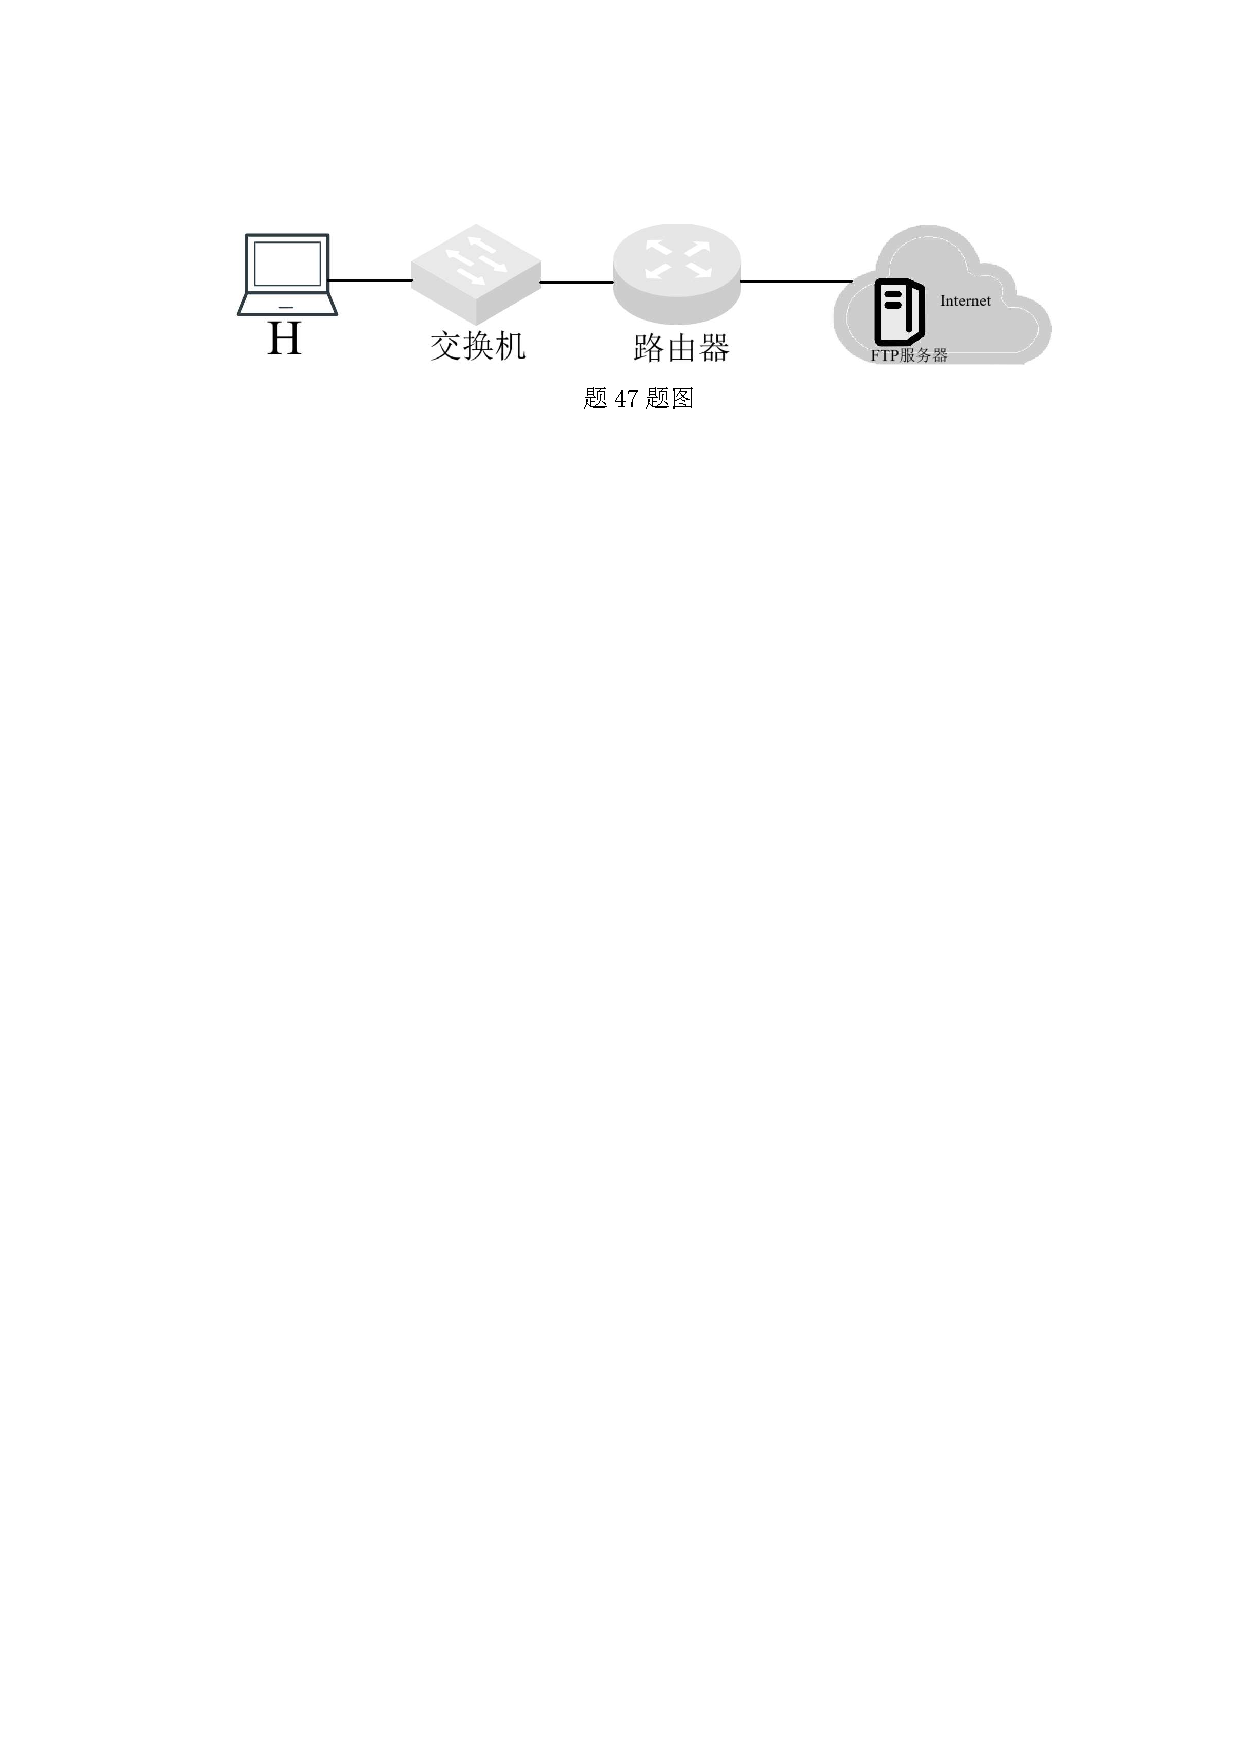
\includegraphics[width=.65\linewidth,height=.4\textheight,keepaspectratio]{../assets/figures/2023-questions-p011-b001.pdf}\end{center}

请回答下列问题：（1）FTP的控制连接是持久的还是非持久的？FTP的数据连接是持久的还是非持久的？H登录FTP服务器时，建立的TCP连接是控制连接还是数据连接？（2）H通过数据连接发送F时，F的第1个字节的序号是多少？在断开数据连接的过程中，FTP服务器发送的第二次挥手ACK段的确认序号是多少？（3）H通过数据连接发送F时，当H收到确认序号为2101的确认段时，H的拥塞窗口调整为多少？收到确认序号为7101的确认段时，H的拥塞窗口调整为多少？（4）H从请求建立数据连接开始，到确认F已被服务全部接收为止，至少需要多长时间？期间应用层数据的平均发送速率是多少？

\end{document}
